%%&program=xelatex
%&encoding=UTF-8 Unicode
% SVN keywords
% $Author$
% $Date$
% $Revision$
% $URL$
\documentclass[a4paper,12pt]{article}      % Comments after  % are ignored
%\usepackage{hyperref}                 % For creating hyperlinks in cross references
%
\usepackage{ifxetex}% for XELATEX, or PDFlatex
\usepackage{ifplatform} 
%
\ifxetex
	\usepackage{polyglossia} \setmainlanguage{portuges}
	\usepackage{fontspec}
	\ifwindows
		\setmainfont[Ligatures=TeX]{Garamond}
		\setsansfont[Ligatures=TeX]{Gill Sans MT}
		\setmonofont{Consolas}		
%		\setmonofont[Scale=MatchLowercase]{Courier}
	\fi
	\iflinux
		\setmainfont[Ligatures=TeX]{Linux Libertine O}
		\setsansfont[Ligatures=TeX,Scale=MatchLowercase]{Linux Biolinum}
		\setmonofont[Scale=MatchLowercase]{Courier}
	\fi
	\ifmacosx
	% add settings
	% Use xelatex -no-shell ...
		\setmainfont[Ligatures=TeX]{Garamond}
		\setsansfont[Ligatures=TeX]{Helvetica}
		\setmonofont{Consolas}
	\fi
	\usepackage{xcolor,graphicx} 
\else
	\usepackage[portuguese]{babel}
	%\usepackage[latin1]{inputenc}
	\usepackage[utf8]{inputenc}
	\usepackage[T1]{fontenc}
	\usepackage{graphics}                 % Packages to allow inclusion of graphics
	\usepackage{color}                    % For creating coloured text and background
\fi

\usepackage{enumitem}
\setlist{nolistsep}
\usepackage{amsmath,amssymb,amsfonts} % Typical maths resource packages

\oddsidemargin 0cm
\evensidemargin 0cm

\pagestyle{myheadings}         % Option to put page headers
                               % Needed \documentclass[a4paper,twoside]{article}
\markboth{{MEFT}}
{{\small\it \protect\input{../../LIFE.txt}}}

\addtolength{\hoffset}{-0.5cm}
\addtolength{\textwidth}{2.5cm}
\addtolength{\topmargin}{-1.5cm}
\addtolength{\textheight}{3cm}

%\textwidth 15.5cm
%\topmargin -1.5cm
\setlength{\parindent}{0pt}
\setlength{\parskip}{1ex  plus  0.5ex  minus  0.2ex}
%\parindent 0.5cm
%\textheight 25cm
%\parskip 1mm


% Math macros
\newcommand{\ud}{\,\mathrm{d}} 
\newcommand{\HRule}{\rule{\linewidth}{0.5mm}}

\author{Prof. Bernardo B. Carvalho} 

%%%%, Bernardo Brotas Carvalho\\bernardo@ipfn.ist.utl.pt} 
\date{ Outubro 2012} 

\begin{document} 

	\includegraphics[width=0.2\textwidth]{../../logo-ist}%\\[1cm]  %%  Logo_IST_color

	\HRule \\[0.5cm]
	{ \huge \sf  \textsc{Medição da Velocidade da Luz} }\\[0.4cm] % \bfseries 
	{ \large \bfseries em diferentes materiais homogéneos e isotrópicos}\\
%	{ \large \bfseries Procedimento Experimental}\\
	\HRule \\%[0.5cm]


\section{\sf Introdução}
Em muitas das experiências descritas na literatura para determinacão da velocidade da luz foram utilizados feixes luminosos pulsados (ou modulados), que percorrem determinados trajetos de maior ou menor comprimento (um exemplo é a Fig. \ref{fig:Fizeau}). 
No presente trabalho, utiliza-se como fonte luminosa um díodo (LED) que emite radiação  visível com um comprimento de onda (c.d.o.) na zona do vermelho. A intensidade da luz emitida pelo díodo, $I_{\textrm{diodo}}(t)$, é \emph{modulada em amplitude} (AM, do inglês \emph{amplitude modulation}), através da aplicação de uma tensão de alimentação sinusoidal de frequência $f_{\textrm{mod}}=50$ MHz, de acordo com a expressão

\begin{equation*}
	\label{eq:f_am}
		I_{\textrm{diodo}}(t) = A_0 (1+ \sin ( 2\pi \cdot 50\times 10^6 \, t))/2
%		}_\text{Amplitude Modulada} \cdot \sin ( 2\pi \cdot f_{luz} \, t)
\end{equation*}
%A(t) \cdot \sin ( 2\pi \cdot f_{luz} \, t) = \underbrace{

\begin{figure}
	[ht!b]  \centering 
	\includegraphics[width=0.5\textwidth]{Fizeau}
	\caption{Esquema do aparelho (Roda de Fizeau) para determinar a velocidade da luz utilizado por Fizeau em 1849. \label{fig:Fizeau}} 
\end{figure}

%\section{\sf Introdução}

\newpage
\section{\sf Base do Método}
No presente trabalho, o feixe luminoso proveniente do LED emissor é forçado a percorrer um determinado trajeto de comprimento $L$, sendo em seguida a sua intensidade  detetada por um fotodíodo receptor (Fig. \ref{fig:Montagem}). O sistema solidário de espelhos $E_1\,, E_2$ pode deslocar-se ao longo de uma calha graduada,
sendo assim possível variar o comprimento do trajeto. Os
sinais de amplitude impostos ao emissor e captados no receptor são registados\footnote{Depois de uma deteção \emph{heteródina}, em que a frequência modulada é desviada de \\ 
$f_{\textrm{bat}}=$50.050 MHz -- 50 MHz  = 50 kHz. Esta operação permite a utilização de um osciloscópio simples de banda de frequências mais estreita.} 
nos canais de um osciloscópio funcionando em modo “XY” (sem base de tempo).

\begin{figure}[htb] 
 \centering 
	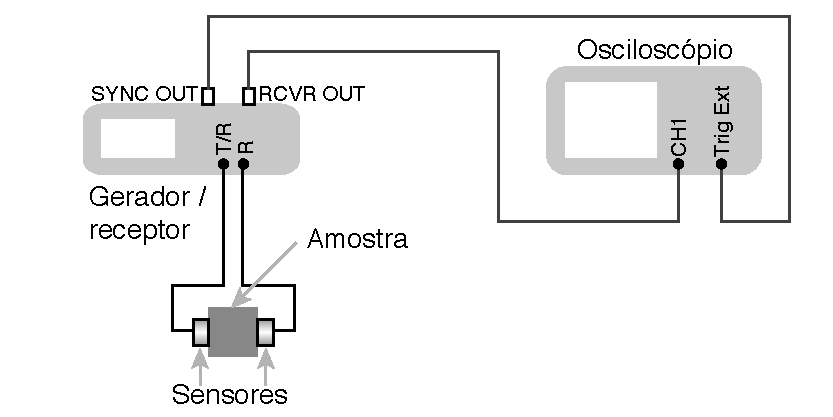
\includegraphics[width=01.0\textwidth]{esquema}
	\caption{Montagem para determinação da velocidade da luz. \label{fig:Montagem}} 
\end{figure}



Em ambos os canais X e Y (vertical e horizontal) a frequência é a mesma\footnote{Os sinais são \emph{coerentes}, pois provêm da mesma fonte.}. No caso mais geral em que os sinais não estão em fase um com o outro, o padrão visualizado no osciloscópio é uma \emph{figura de Lissajous}, neste caso uma elipse (Fig. \ref{fig:fase}), com um parâmetro $\delta$ dado pela equação geral:
\begin{equation}
	\label{eq:elipse}
	\sin^2 \delta = \frac{A_x^2}{A_{x0}^2} + \frac{A_y^2}{A_{y0}^2} - \frac{2 A_y\,A_x}{A_{y0}\,A_{x0}} \cos  \delta
\end{equation}
sendo $A_x(t)$ o sinal de intensidade captado no emissor,  $A_y(t)$ o sinal
proveniente do recetor, $A_{x0}$, $A_{y0}$ as respectivas amplitudes e $\delta$ a desfasagem entre os dois sinais. A desfasagem relativa entre os sinais (e, logo, o ângulo $\delta$) varia com o comprimento do trajecto $L$ percorrido pelo raio luminoso. Este efeito traduz-se numa variação da forma da elipse observada.  A elipse pode degenerar em retas quando os dois sinais estiverem em fase, $\delta = 2n\pi$ (nos quadrantes ímpares)  ou em oposição de fase, $\delta = (2n+1)\,\pi$ (nos quadrantes pares). 

\begin{figure}
	[htb]  \centering 
	\includegraphics[width=0.8\textwidth]{osci_fase}
	\caption{Figuras de Lissajous observadas no osciloscópio. À esquerda: sinais em fase; centro: sinais com uma dada desfasagem $\theta$; direita: sinais em oposição de fase.  \label{fig:fase}} 
\end{figure}

\subsection{\sf Velocidade da luz no ar}
Neste trabalho, a velocidade da luz é calculada a partir da determinação do comprimento do
caminho suplementar $\Delta L= 2\,\Delta z_0$ (ver fig. \ref{fig:Montagem}) que a luz tem de percorrer para que se passe de uma
situação em que os sinais estão em fase à situação contígua de
 oposição de fase (ou vice-versa). Por definição, para passar de uma situação à outra é necessário que o tempo gasto no percurso suplementar corresponda a metade de um período. Assim, a luz percorre essa distância num intervalo de tempo $\Delta t$ igual a metade do período do sinal modulante, ou seja $\Delta t=T/2=1/(2\cdot50\,\textrm{MHz})= 10\,\textrm{ns}$. 
No trajecto da luz no ar teremos a seguinte expressão para a sua velocidade:
\begin{equation}
	\label{eq:vc}
	c_{ar} = \frac{\Delta L}{\Delta t}=\frac{2\,\Delta z_0}{T/2} 
\end{equation}


\subsection{\sf Velocidade da luz em meios sólidos e líquidos}
 O índice de refração de um meio material $1$ em relação a outro meio $0$, para um dado comprimento de onda, é definido\footnote{Esta definição só é válida se as condutividades elétricas dos meios $0$ e $1$ forem nulas, ou seja, nos \emph{dielétricos} perfeitos.}
 como o quociente entre as velocidades de propagação da luz nos meios $0$ e $1$:

 \begin{equation}
	\label{eq:index}
	n_1 \equiv \frac{c_0}{c_1}  = \frac{\frac{1}{\sqrt{\varepsilon_0 \, \mu_0}} }{\frac{1}{\sqrt{\varepsilon_1 \, \mu_1}} } =
		\sqrt{\frac{\varepsilon_1 \, \mu_1}{\varepsilon_0 \, \mu_0}} = \sqrt{\varepsilon_r \, \mu_r}
\end{equation}

Nesta expressão $\varepsilon_0$, $\varepsilon_1$ ,	 $\mu_0$, $\mu_1$ são as constantes dielétricas e as permeabilidades magnéticas respetivamente do meios $0$ e $1$ e $\varepsilon_r$, $\mu_r$    as relativas $(\varepsilon_1= \varepsilon_r\, \varepsilon_0)$.

\begin{figure}[h!tb]  
	\centering 
	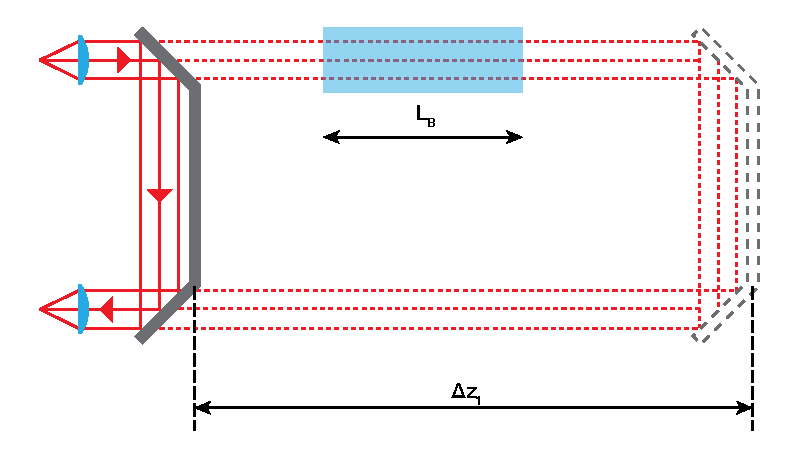
\includegraphics[width=0.8\textwidth]{esquema2}
	\caption{Montagem para determinar índices de refração em sólidos e líquidos. \label{fig:Montagem_bloco}} 
\end{figure}

Se no percurso do feixe luminoso interpusermos um bloco transparente de material sólido ou líquido de comprimento $l_B$ (Fig. \ref{fig:Montagem_bloco}), o comprimento suplementar necessário $\Delta L$ entre as posições de fase e oposição de fase vai variar. De facto, uma vez que as velocidades da luz nesse material e no ar são diferentes, a desfasagem introduzida por uma dada espessura de material também difere da desfasagem causada pela mesma espessura de ar. É pois necessário contabilizar em separado o tempo necessário para percorrer o bloco de espessura $l_B$ à velocidade $c_B$ e o restante comprimento de ar à velocidade $c_{ar}$, obtendo-se a expressão

\begin{equation}
	\label{eq:vc_bloco}
	{T/2}  = \frac{2\,\Delta z_1 - l_B}{c_{ar}}  +  \frac{l_B}{c_{B}}
\end{equation}
em que $\Delta z_1$ é a nova posição em que se regista passagem de fase para oposição de fase (ou vice-versa). A partir daqui calcula-se a velocidade $c_{B}$.  

Pode ainda obter-se o valor do índice de refração $n_{B}$ com a ajuda de (\ref{eq:vc}) e (\ref{eq:index}):

\begin{align}
	\label{eq:n_bloco}
	{T/2}  = \frac{2\,\Delta z_0}{c_{ar}}  &=  \frac{2\,\Delta z_1 }{c_{ar}} -   \frac{l_B}{c_{ar}}  +  \frac{l_B}{c_{B}} \nonumber \\ 
	\frac{2\,(\Delta z_0- \Delta z_1 )}{c_{ar}}  &= -   \frac{l_B}{c_{ar}}  +  \frac{l_B}{c_{B}} \nonumber \\
	\frac{2\,(\Delta z_0- \Delta z_1 )}{l_B} &= -1 +  \frac{c_{ar}}{c_{B}} \nonumber \\
	n_{B} &= 1 +  \frac{2\,(\Delta z_0- \Delta z_1 )}{l_B} 
\end{align}

Neste trabalho, serão  determinados os índices de refração e a velocidade da luz em  dois meios materiais, a resina acrílica e a água. 
 


\newpage
\section{\sf Protocolo Experimental}
\subsection{\sf Material utilizado}

\begin{enumerate}
\setlength{\itemsep}{0mm}
\item Unidade de emissão de luz  (com amplitude modulada por um sinal de frequência 50 MHz) e de recepção.
% (díodos receptor) amplitude modulada por um sinal de frequência $50\,MHz$)(.
\item Duas lentes plano-cilíndricas.
\item Conjunto de dois espelhos planos para inversão do sentido de propagação da luz.
\item Calha graduada.  
\item Bloco de vidro acrílico transparente.
\item Dois tubos com cerca de 1 metro de comprimento para conter água ou ar. 
\item Osciloscópio de dois canais a funcionar em modo XY.
\end{enumerate}

\subsection{\sf Procedimento Experimental}
\subsubsection{\sf Regulação da montagem}
 
\begin{enumerate}
\setlength{\itemsep}{0mm}
\item Comece por verificar se a montagem óptica está devidamente alinhada. Retire ambas as lentes da montagem. Posicione e ajuste a lente junto ao LED emissor e, usando um alvo difusor (papel vegetal, por exemplo), observe a forma da mancha luminosa ao longo do percurso óptico, de modo a tentar obter um diâmetro constante (feixe de raios paralelos, ou colimado).
\item Ainda sem a segunda lente, verifique que a mancha luminosa está centrada com  a janela do díodo receptor.
\item Coloque agora a lente no lado do díodo receptor e, ajustando-a, alinhe o foco do feixe convergente no seu centro. 
\item Ajuste os parafusos dos espelhos de forma a maximizar a amplitude do sinal  recebido.
\item Coloque os espelhos na posição zero da escala. Rodando o botão da unidade que ajusta electronicamente a diferença de fase entre os dois sinais, obtenha uma reta dos quadrantes (ím)pares . 
\end{enumerate}

\subsubsection{\sf Velocidade de propagação da luz no ar}
\begin{enumerate}
\item Desloque os espelhos sobre a calha e observe a modificação da figura no ecrã do 
osciloscópio, em particular nas posições que correspondem a que os sinais recebidos estejam 
desfasados de $\delta=\pi/2$ (quadratura) e em oposição de fase, $\delta=\pi$. Para esta última situação, registe a 
nova posição dos espelhos e o intervalo de incerteza $e_z$  entre o qual os sinais parecem estar ainda em 
oposição de fase. 
\item Repita o procedimento para cada observador. 
\item Calcule a velocidade de propagação da luz no ar, a sua incerteza e o desvio à exatidão\footnote{O valor $c_{ar}$ é muito próximo de $c_{vacuo}$ = 299 792 458 m/s, que é uma constante exacta do Sistema Internacional de Medidas. O índice de refração do ar para a luz visível é $n_{ar}=1.000293$.}. 
\end{enumerate}

\subsubsection{\sf Velocidade de propagação da luz no vidro acrílico}
\begin{enumerate}
\item Verifique novamente se no zero da posição dos espelhos os sinais estão em fase. Coloque o bloco de vidro 
acrílico no percurso do feixe incidente, de modo a que incida perpendicularmente à face e usando o percurso 
mais longo no vidro acrílico. 
\item Meça a posição e a incerteza correspondente dos espelhos para que os dois sinais detetados estejam em oposição em fase. 
\item Repita a medição pelo menos 
duas vezes.
\item Calcule o índice de refração obtido para o vidro acrílico, $n_{vidro}$, pela expressão (\ref{eq:n_bloco}),  e a sua incerteza. 
\item Calcule o valor da velocidade da luz no vidro.
\end{enumerate}

\subsubsection{\sf Velocidade de propagação da luz na água}
\begin{enumerate}
\item Verifique a fase na posição inicial. Coloque o tubo vazio  nos suportes de modo a que o feixe incidente entre perpendicularmente à face. Pode desmontar o tubo com ar para medir o comprimento interno do trajeto no ar/água.
\item Registe a posição dos espelhos $z_{0_{ar}}$ que produz um sinal em oposição de fase. 
\item Repita estas medidas para o tubo cheio de água e obtenha o valor correspondente $z_{1_{agua}}$. 
\item Calcule o valor do índice de refração $n_{agua}$ obtido, a sua incerteza e o desvio à exatidão\footnote{O valor tabelado é $n_{agua}=1.3330$.}. 
\item Comente a precisão do valor da velocidade de propagação da luz obtida nos 
diferentes meios.
\end{enumerate}

\end{document} 